For at teste om mutationen fungerer korrekt, printes i dette eksempel et skema før og efter en mutation, samt de tilfældige dage og lektioner, der tilfældigt blev valgt. I eksemplet ses det, at de tilfældige lektioner blev 2 og 4, og de tilfældige dage blev 3 og 0. Da der tælles fra 0, svarer det til den 3. lektion på 4. dag, der skal byttes med den 5. lektion på 1. dag.

\begin{figure}[!ht]
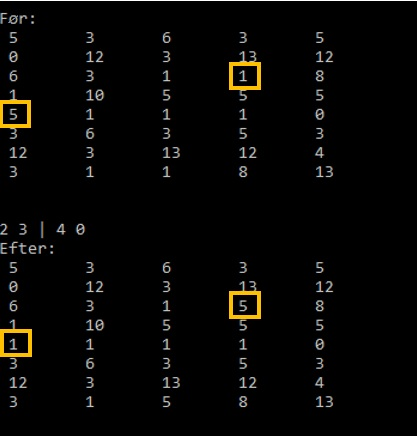
\includegraphics{partials/graphics/mutationbevis.png}
\label{fig:mutationsbevis}
\end{figure}

På figuren ses det at netop de nævnte lektioner er blevet flyttet, så mutationen fungerer som den skal.